\acresetall
\chapter*{DBA Virtualization to Enable PON Multi-Tenancy}

%%%%%%%%%%%%%%%%%%%%%%%%%%%%%%%%%%%%%%%%%%%%%%%%%%%%%%%%%%
%%%%%%%%%%%%%%%%%%%%%%%%%%%%%%%%%%%%%%%%%%%%%%%%%%%%%%%%%%
%%%%%%%%%%%%%%%%%%%%%%%%%SECTION%%%%%%%%%%%%%%%%%%%%%%%%%%
%%%%%%%%%%%%%%%%%%%%%%%%%%%%%%%%%%%%%%%%%%%%%%%%%%%%%%%%%%
%%%%%%%%%%%%%%%%%%%%%%%%%%%%%%%%%%%%%%%%%%%%%%%%%%%%%%%%%%
% \subsubsection{Virtual \ac{DBA} enabling true \ac{PON} multi-tenancy}
% \label{subsection:vDBA}
The current scene on the broadband/mobile operators' market is an oligopoly, where novelty is limited by the market development policies of a hand-full of operators. The cost of entering this market is unaffordably high for smaller service providers who could bring considerable revenue to the access market by introducing new services. Sharing the last mile of access networks, which is the most \ac{CapEx} demanding part, can dramatically reduce the required initial investment and facilitate market entrance for new operators. However, the current sharing methods, especially in fixed access networks, operate at too a high-level (e.g., \ac{VULA}) where they are not capable of providing enough control over the service provided to the customers \cite{7592399}. Other proposals exist for low-level access, which typically translates in assigning a dedicated wavelength to a second operator. However, besides being inefficient, they are currently hindered by the fact that multi-wavelength \ac{PON} (e.g., \ac{NG-PON2}) has not been widely deployed due to its high cost (see \autoref{Back:Sec:PON}). Therefore, we propose a new sharing technique for \acp{PON}, which meets the above-mentioned methods in the halfway by providing frame-level scheduling control for the operators while being more affordable and easier to attract new entrants \cite{7936877}.
% \section{Virtual \ac{DBA} for multi-operator/service convergence}
 \acp{PON} are cost-effective solutions for providing highly capillary connectivity to heterogeneous services, serving residential users, mobile cloud-RAN, and next generations services. Examples are haptic feedback for medical applications or reliable and timely exchange of control messages and camera streams in automotive applications. Some of these new services will, however, require stricter \ac{QoS} than simple committed rate assurance, including latency and jitter targets. 

From a \ac{PON} perspective, this requires the development of new \ac{DBA} mechanisms, which have become the focus of recent research. Virtualization of the \ac{DBA} process can provide strict-\ac{QoS} (i.e., capacity, latency, and jitter assured services) over a multi-tenant environment. \ac{PON} networks are considered a strong candidate for providing networks' services to 5G networks and beyond \cite{8412589}. The lack of control over scheduling remains the single most significant technological barrier in \ac{PON} sharing. In conventional \acp{PON}, the \ac{DBA} is typically implemented as a hard-coded function on the \ac{OLT} and cannot be customized to meet the diverse demand of the tenant \acp{VNO} providing heterogeneous services. As mentioned in \autoref{Back:Sec:Virtualazation}, numerous initiatives (including CORD \cite{7588276}, and \ac{BBF}'s TR-370 \cite{bbfTR370}) are proposing solutions based on network virtualization technology.
In the next section, we will elaborate on the importance of providing scheduling control for the operators and describe the proposed \ac{vDBA} concept and architecture.
\begin{figure}%[htbp]
% \vspace{-3mm}
\centering
 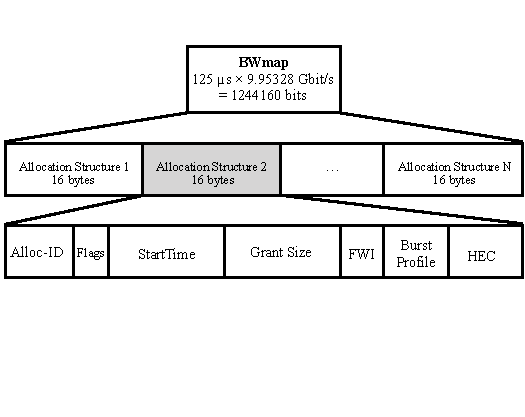
\includegraphics[width=0.8\columnwidth]{Figures/BMap.pdf}
\caption{XGS-\ac{PON} \ac{BMap} allocation structure format}
\vspace{-2mm}
\label{BMap}
\end{figure}
\section{DBA Virtualization}
\ac{PON} is a point-to-multipoint optical access technology, which requires scheduling in the upstream transmission to avoid collisions between the data sent by the ONUs. \ac{DBA} is a process that assigns time slots to each \ac{ONU} for upstream transmission. The outcome of the \ac{DBA} process is the transmission schedule for the ONUs, i.e., "\ac{BMap}".  \figureautorefname~\ref{BMap} depicts the format of the XGS-\ac{PON} \cite{G.9807.1} \ac{BMap} partition and an allocation structure. The \ac{BMap} is generated by the OLT and broadcast to all of the ONUs in every 125 microseconds (i.e., the duration of a \ac{PON} frame). The finest granularity allowed for each allocation structure is 16 bytes. Thus, each \ac{BMap} may contain up to 9720 allocation structures for a 10 Gb/s upstream channel. ITU standards identify two \ac{DBA} classifications. The first type is status reporting (SR) \ac{DBA}, which schedules the transmission based on the definite reports of buffer occupancy of the ONUs and generates a precise allocation based on it. The second type is non-status-reporting (NSR) \ac{DBA}, which bases the scheduling on the information acquired from traffic monitoring. The SR \ac{DBA} provides higher precision but imposes some latency due to the exchange of control signals \cite{haran2008importance}.
\begin{figure}%[h]
% \vspace{-7mm}
\centering
\begin{subfigure}{0.41\columnwidth}
 \includegraphics[width=\textwidth]{Figures/dba}
\caption{Conventional \ac{PON}}%
\label{dba}
\end{subfigure}\hfill%
\begin{subfigure}{0.59\columnwidth}
 \includegraphics[width=\textwidth]{Figures/vdba}
\caption{Multi-tenant \ac{PON} with \ac{DBA} Virtualization}%
\label{vdba}
\end{subfigure}\hfill%
\caption{Conventional \ac{PON} vs. Proposed Multi-Service/Tenant \ac{PON}}
\label{DBAvsVDBA}%
% \vspace{-9mm}
\end{figure}
Current \acp{PON} fail to support the diverse range of requirements associated with the next generation of services (for 5G and beyond). For instance, current \acp{PON} cannot be used to provide connectivity between \ac{RRH} and \ac{BBU} in mobile Cloud-RAN applications, as it cannot meet the required delay budget, which is of the order of few hundreds of microseconds \cite{Zhou:18} unless if a static fixed bandwidth is allocated. %Yet, the current \ac{DBA} algorithms that are hard-coded into the OLT are unable to provide such low-latency scheduling solutions. 
Thus, the research community is investigating new \ac{DBA} algorithm designs e.g. predictive \cite{8289443} or unified \acp{vDBA}-Wireless scheduler \cite{Zhou:18}, to provide support for these ultra low-latency services.

\section{\acf{vDBA} }
Figure~\ref{DBAvsVDBA} shows the comparison between today's \ac{PON} and the proposed Multi-Tenant \ac{PON}, which implements the \ac{vDBA} concept. 
In traditional \acp{PON}, a single \ac{DBA} scheme is implemented in the \ac{OLT} hardware (\figureautorefname~\ref{dba}). From hereafter, we shall refer to the \ac{DBA} scheme implemented in hardware as physical \ac{DBA} (PHY-\ac{DBA}). In this architecture, only the \ac{InP} controls the PHY-\ac{DBA} function. Consequently, in a multi-tenancy context, the \acp{VNO} are not able to directly control the \ac{DBA} process for \acp{ONU} associated with their customers/services, in other words, \acp{VNO} cannot schedule themselves the burst allocation of their customers' \acp{ONU}. Proper burst allocation by \ac{DBA} is important to assure strict-\ac{QoS} (in terms of jitter and latency), e.g., for low latency cloud-RAN and other \ac{5G} services. To assure strict-\ac{QoS} services, the \acp{VNO} would have to request and rely on \ac{SLA}'s guarantees (e.g., bandwidth, latency, jitter) to be provided by the \ac{InP}, that would manage its \ac{DBA} to combine the different offered services to the different \acp{VNO}. However, this would be rather static and might not be able to follow some \acp{VNO} requirements. For instance, the \ac{InP} can assign a certain amount of assured bandwidth to each \ac{VNO} and guarantee their \ac{QoS} requirments averaged over a few miliseconds.
 Alternatively, in order to enable direct control of each \ac{VNO} on their own \ac{DBA} process, we propose a Multi-Tenant architecture shown in \figureautorefname~\ref{vdba}. The description below reports the operation of layers that are involved in the \ac{vDBA} process. The Physical layer takes care of framing in the data plane; the \ac{ME} layer receives multiple \ac{vDBA} \acp{BMap}, merging them into one physical \ac{BMap} for the \acp{ONU}; and the \ac{vDBA} layers, operated by the \acp{VNO} compute a \ac{vBMap} for each slice of \ac{OLT} they have access to.
 The \ac{vDBA} operates within a \ac{vOLT}, which is an NFV slice of a physical \ac{OLT} and is associated with a \ac{VNO}. The \ac{vDBA} allows \acp{VNO} to control, for each \ac{T-CONT}, upstream capacity, latency, and jitter in a shared physical \ac{OLT}, thus delivering a\textit{ True Multi-Tenant \ac{PON} solution}. The layers of the \ac{vDBA} architecture are as follow:
 




\begin{itemize}
\item \par{\textbf{Virtual \ac{OLT} layer with \ac{vDBA}}}


This is the layer controlled by the \ac{VNO}, which enables full control over the choice of the most appropriate \ac{vDBA} algorithm to run on the virtual \ac{PON} slice. As shown in \figureautorefname~\ref{vdba}, the \ac{vDBA} generates the \ac{vBMap} for its \ac{PON} slice and delivers it to the \ac{ME}. For \acp{ONU} with strict latency and jitter requirements, this \ac{vBMap} indicates the desired position for each slot allocation. In this way, the \ac{VNO} obtains full control over the upstream capacity scheduling within each frame. The \ac{vDBA} should create a \ac{vBMap} based on the same frame size as the physical \ac{BMap}.
   
    \item \par{\textbf{\acf{ME} Layer}}
    
The \ac{ME} is the core of the multi-tenant \ac{PON} architecture. It is considered the bridge between the \ac{OLT} and \acp{vOLT}. The \ac{ME} replaces the physical \ac{DBA} layer and has two main tasks. Firstly, it relays queue status report messages (BufOcc or report frames) coming from the \acp{ONU} (from specific \acp{T-CONT}) towards the relevant \ac{vOLT}. Secondly, it analyzes the \acp{vBMap} from all \acp{vDBA}, merging them into one physical bandwidth grant (PHY-\ac{BMap}) and sent it to all \acp{ONU}. It should be noticed that for cloud-RAN, which has very strict latency and jitter constraints, but for which the \ac{BBU} knows in advance the upstream capacity allocation, BufOcc (normally generated by the \ac{ONU}), could be generated directly by the \ac{BBU}, and sent to the \ac{vDBA}, in order to eliminate the latency associated with the queue reporting mechanism \cite{ituG.front, 6886953}. 
% \towrite{Need to refr to cooperative dba ntt 0fc 2014/7 paper also ITU standard} 
The \ac{ME} is controlled by the \ac{InP}. The \ac{ME} should send PHY-\ac{BMap} to all \ac{ONU} every frame (e.g., every 125 microseconds). \acp{vDBA} however are not required to submit a \ac{vBMap} every frame. It should be noted that in order to reduce the latency between the \ac{TC} layer, \ac{ME}, and \ac{vDBA}, these might be physically co-located, for example in a system-on-chip architecture.

\item \par{\textbf{\acf{TC} Layer}} 

The \ac{TC} layer implements the framing and other data plane functions. The \ac{InP} is in charge of controlling this layer and will manage the different wavelength channels in a multi-wavelength \ac{PON}. 
\end{itemize}





\section{Quality of Service Classes} There should be at least three classes of service for the \acp{T-CONT} in the \ac{vDBA} scheme:
\begin{itemize}
    \item Strict-\ac{QoS} \ac{T-CONT}, which defines latency and jitter constraints in addition to AIR/PIR. The \ac{ME} is required to consider the specific slot allocation (i.e., start and stop position of each allocation) only for this service class.
    \item \ac{QoS} \ac{T-CONT} which only define assured rate - AIR (which is met within the few milliseconds described in existing standards) 
    \item Non-assured \ac{T-CONT}, which is allocated capacity when there is space available.
\end{itemize}

 Whenever a new service with strict latency and jitter is requested from a customer to the \ac{VNO}, it allocates a new dedicated strict-\ac{QoS} \ac{T-CONT}, where the desired level of latency, jitter, and availability are defined together with the capacity needed (e.g., in terms of committed rate). The \ac{vDBA} sends the request to the \ac{ME}, which can accept or reject it, depending on the available capacity. Where there is overlap between \acp{vBMap} from different \acp{VNO}, the \ac{ME} can move the slots allocation when generating the physical \ac{BMap} with respect to their request in the \ac{vBMap}, as far as the allocated slots still respect the capacity and maximum latency and jitter required by the \ac{ONU}. In the case where the service requiring the strict-\ac{QoS} has a fixed transmission rate (or fixed within a given time length of several frames duration), there can be an additional negotiation phase during the initial allocation of the \ac{T-CONT}, to mitigate the issue above. The \ac{vDBA} can propose a slot allocation, which shall then remain constant across several other frames. The \ac{ME} can either accept, reject, or propose modifications to the \ac{T-CONT} allocation, e.g., in a way that would fit within the frame allocation (i.e., considering other similar services already allocated). The process will iterate until an agreement is reached or the service is rejected.



\section{Inter-Operator Excess Capacity Sharing}
The \ac{ME} analyzes the \acp{vBMap} from all \acp{vDBA}, merging them into one physical \ac{BMap}. Within the context of XGS-PON, the \ac{ME} layer is responsible for merging \acp{vBMap} generated from virtual \acp{DBA}. Each \ac{VNO} has been dedicated a pre-negotiated share of every frame which could utilize as it sees fit. However, in the case when one or more \acp{VNO} do not have enough demand for transmission from their \acp{ONU}, the excess capacity could be shared with other \acp{VNO} that potentially have excess demand for bandwidth.

\begin{figure}%[h]
% \vspace{-7mm}
\centering
\begin{subfigure}{0.48\columnwidth}
 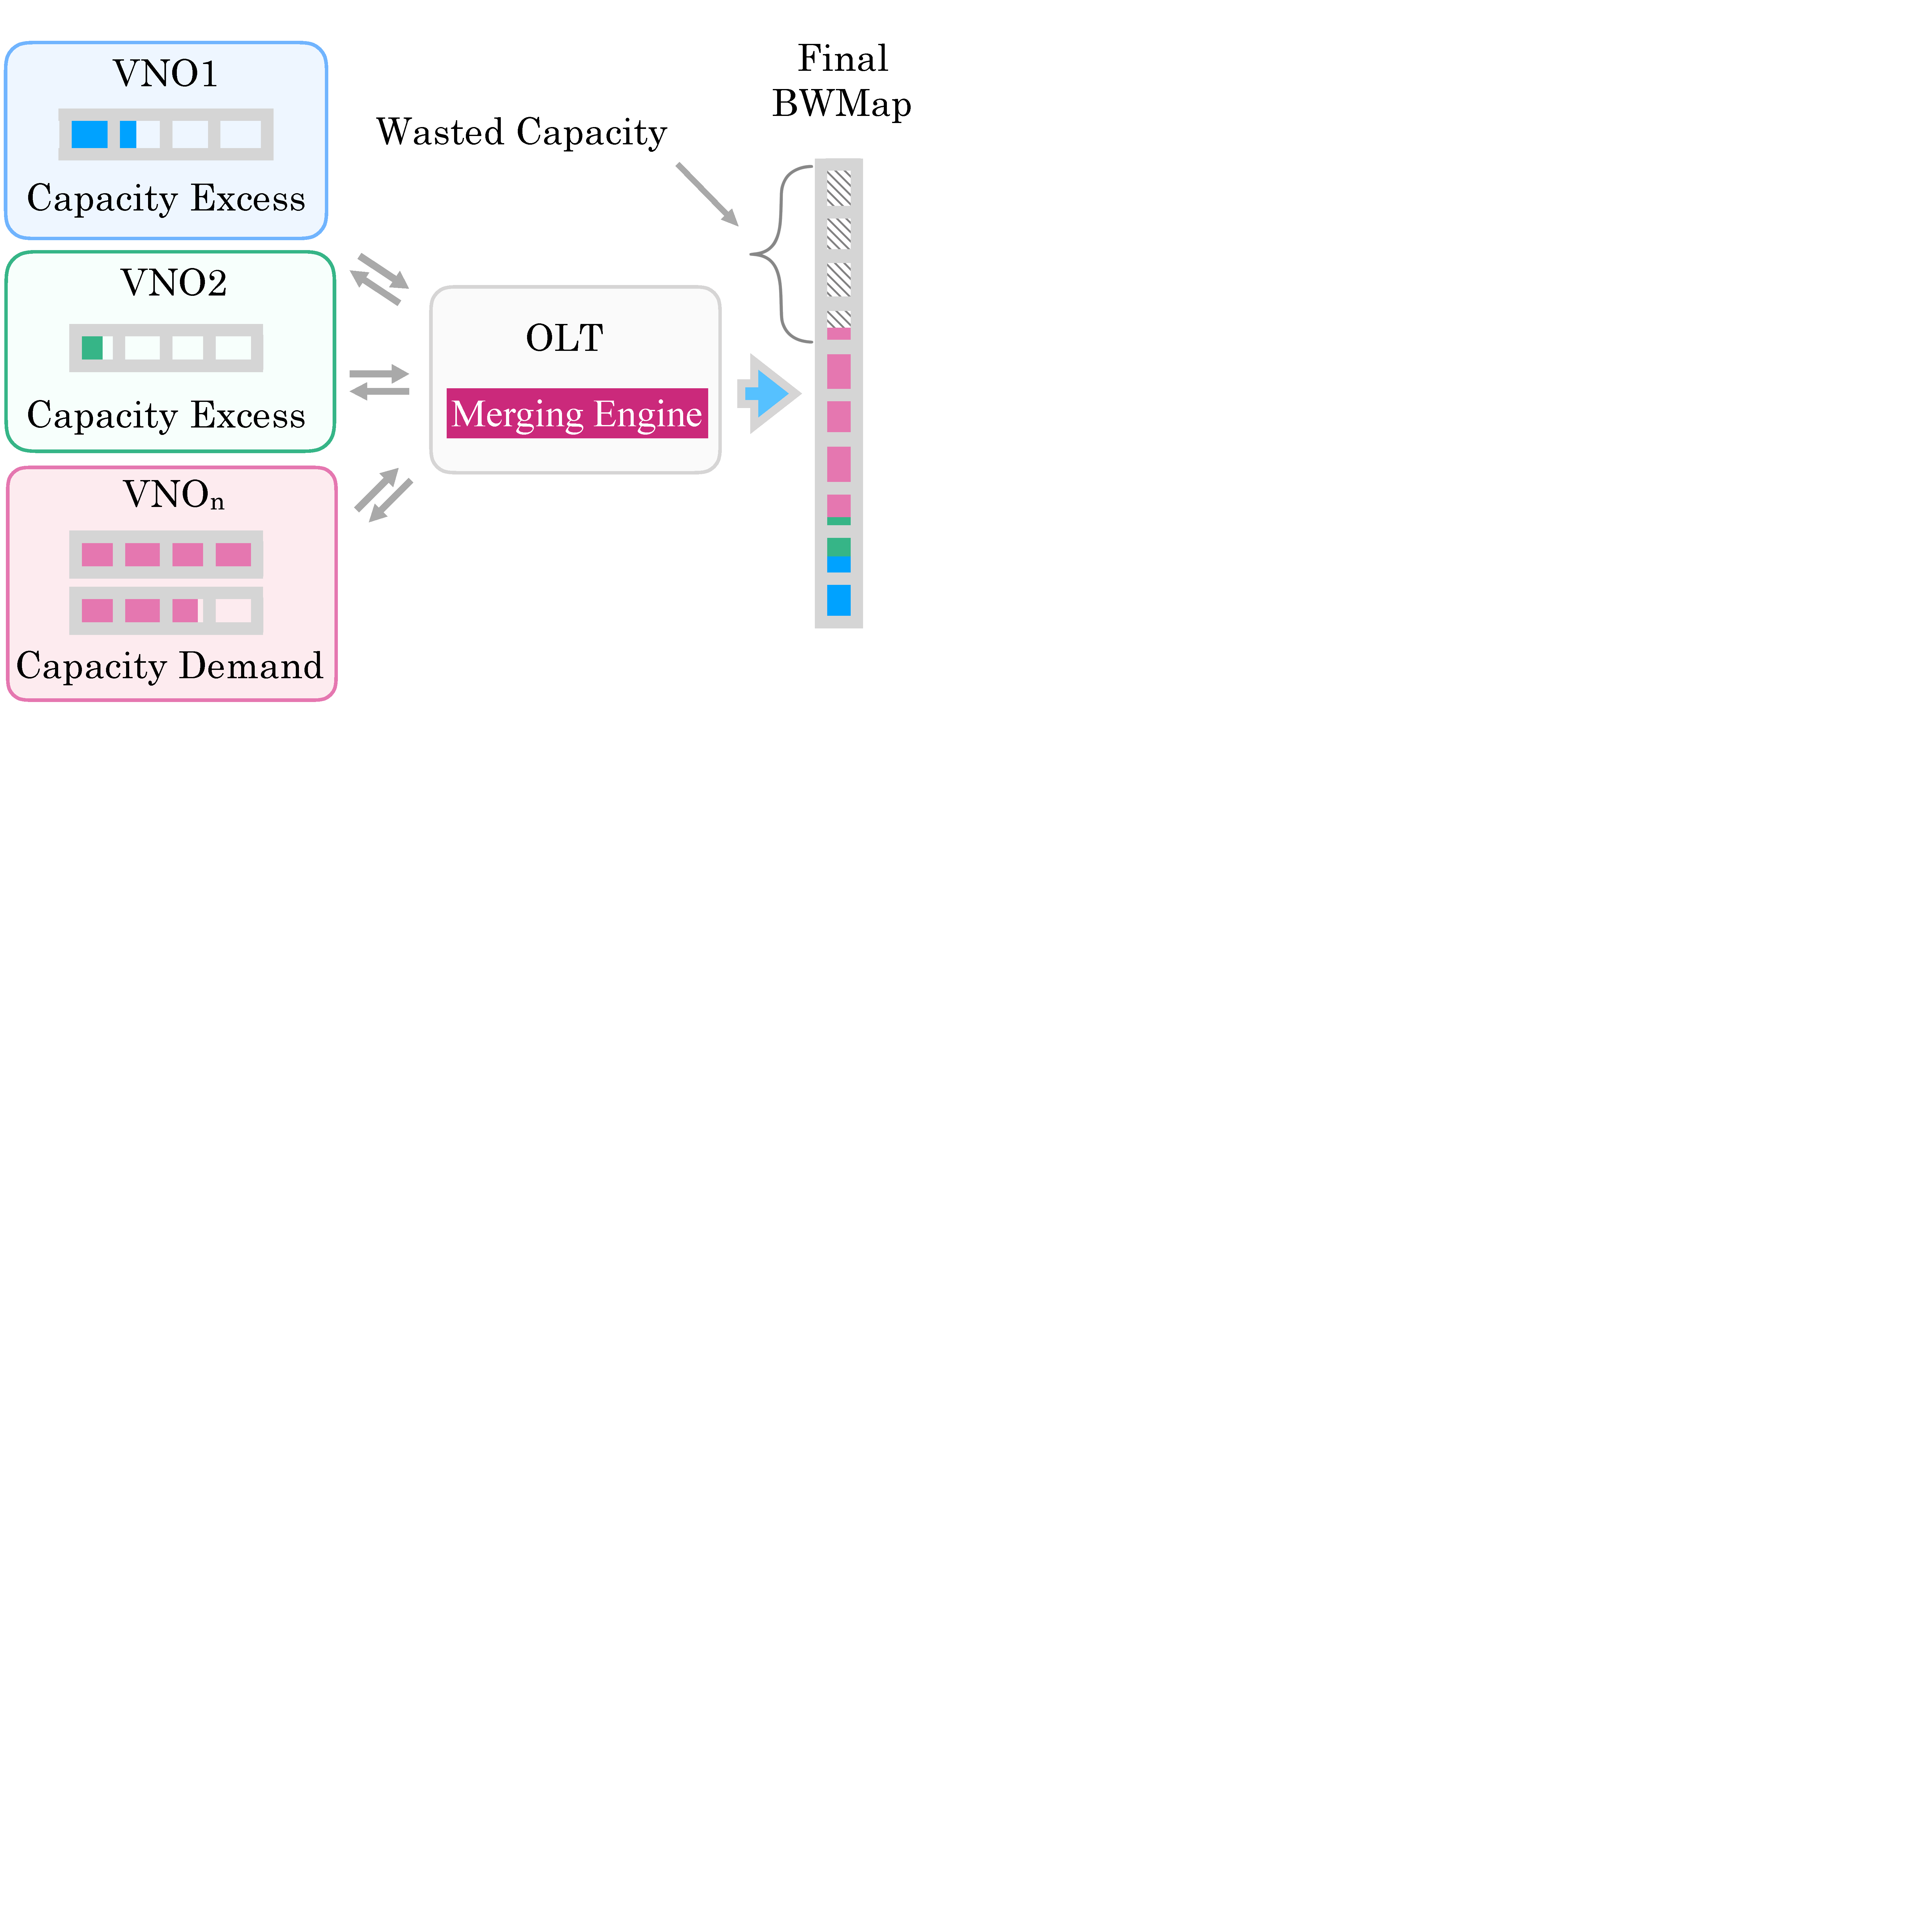
\includegraphics[width=\textwidth]{Figures/non-sharing.pdf}
\caption{Excess Non-Sharing Policy}%
\label{nonsharing_p}
\end{subfigure}\hfill%
\begin{subfigure}{0.48\columnwidth}
 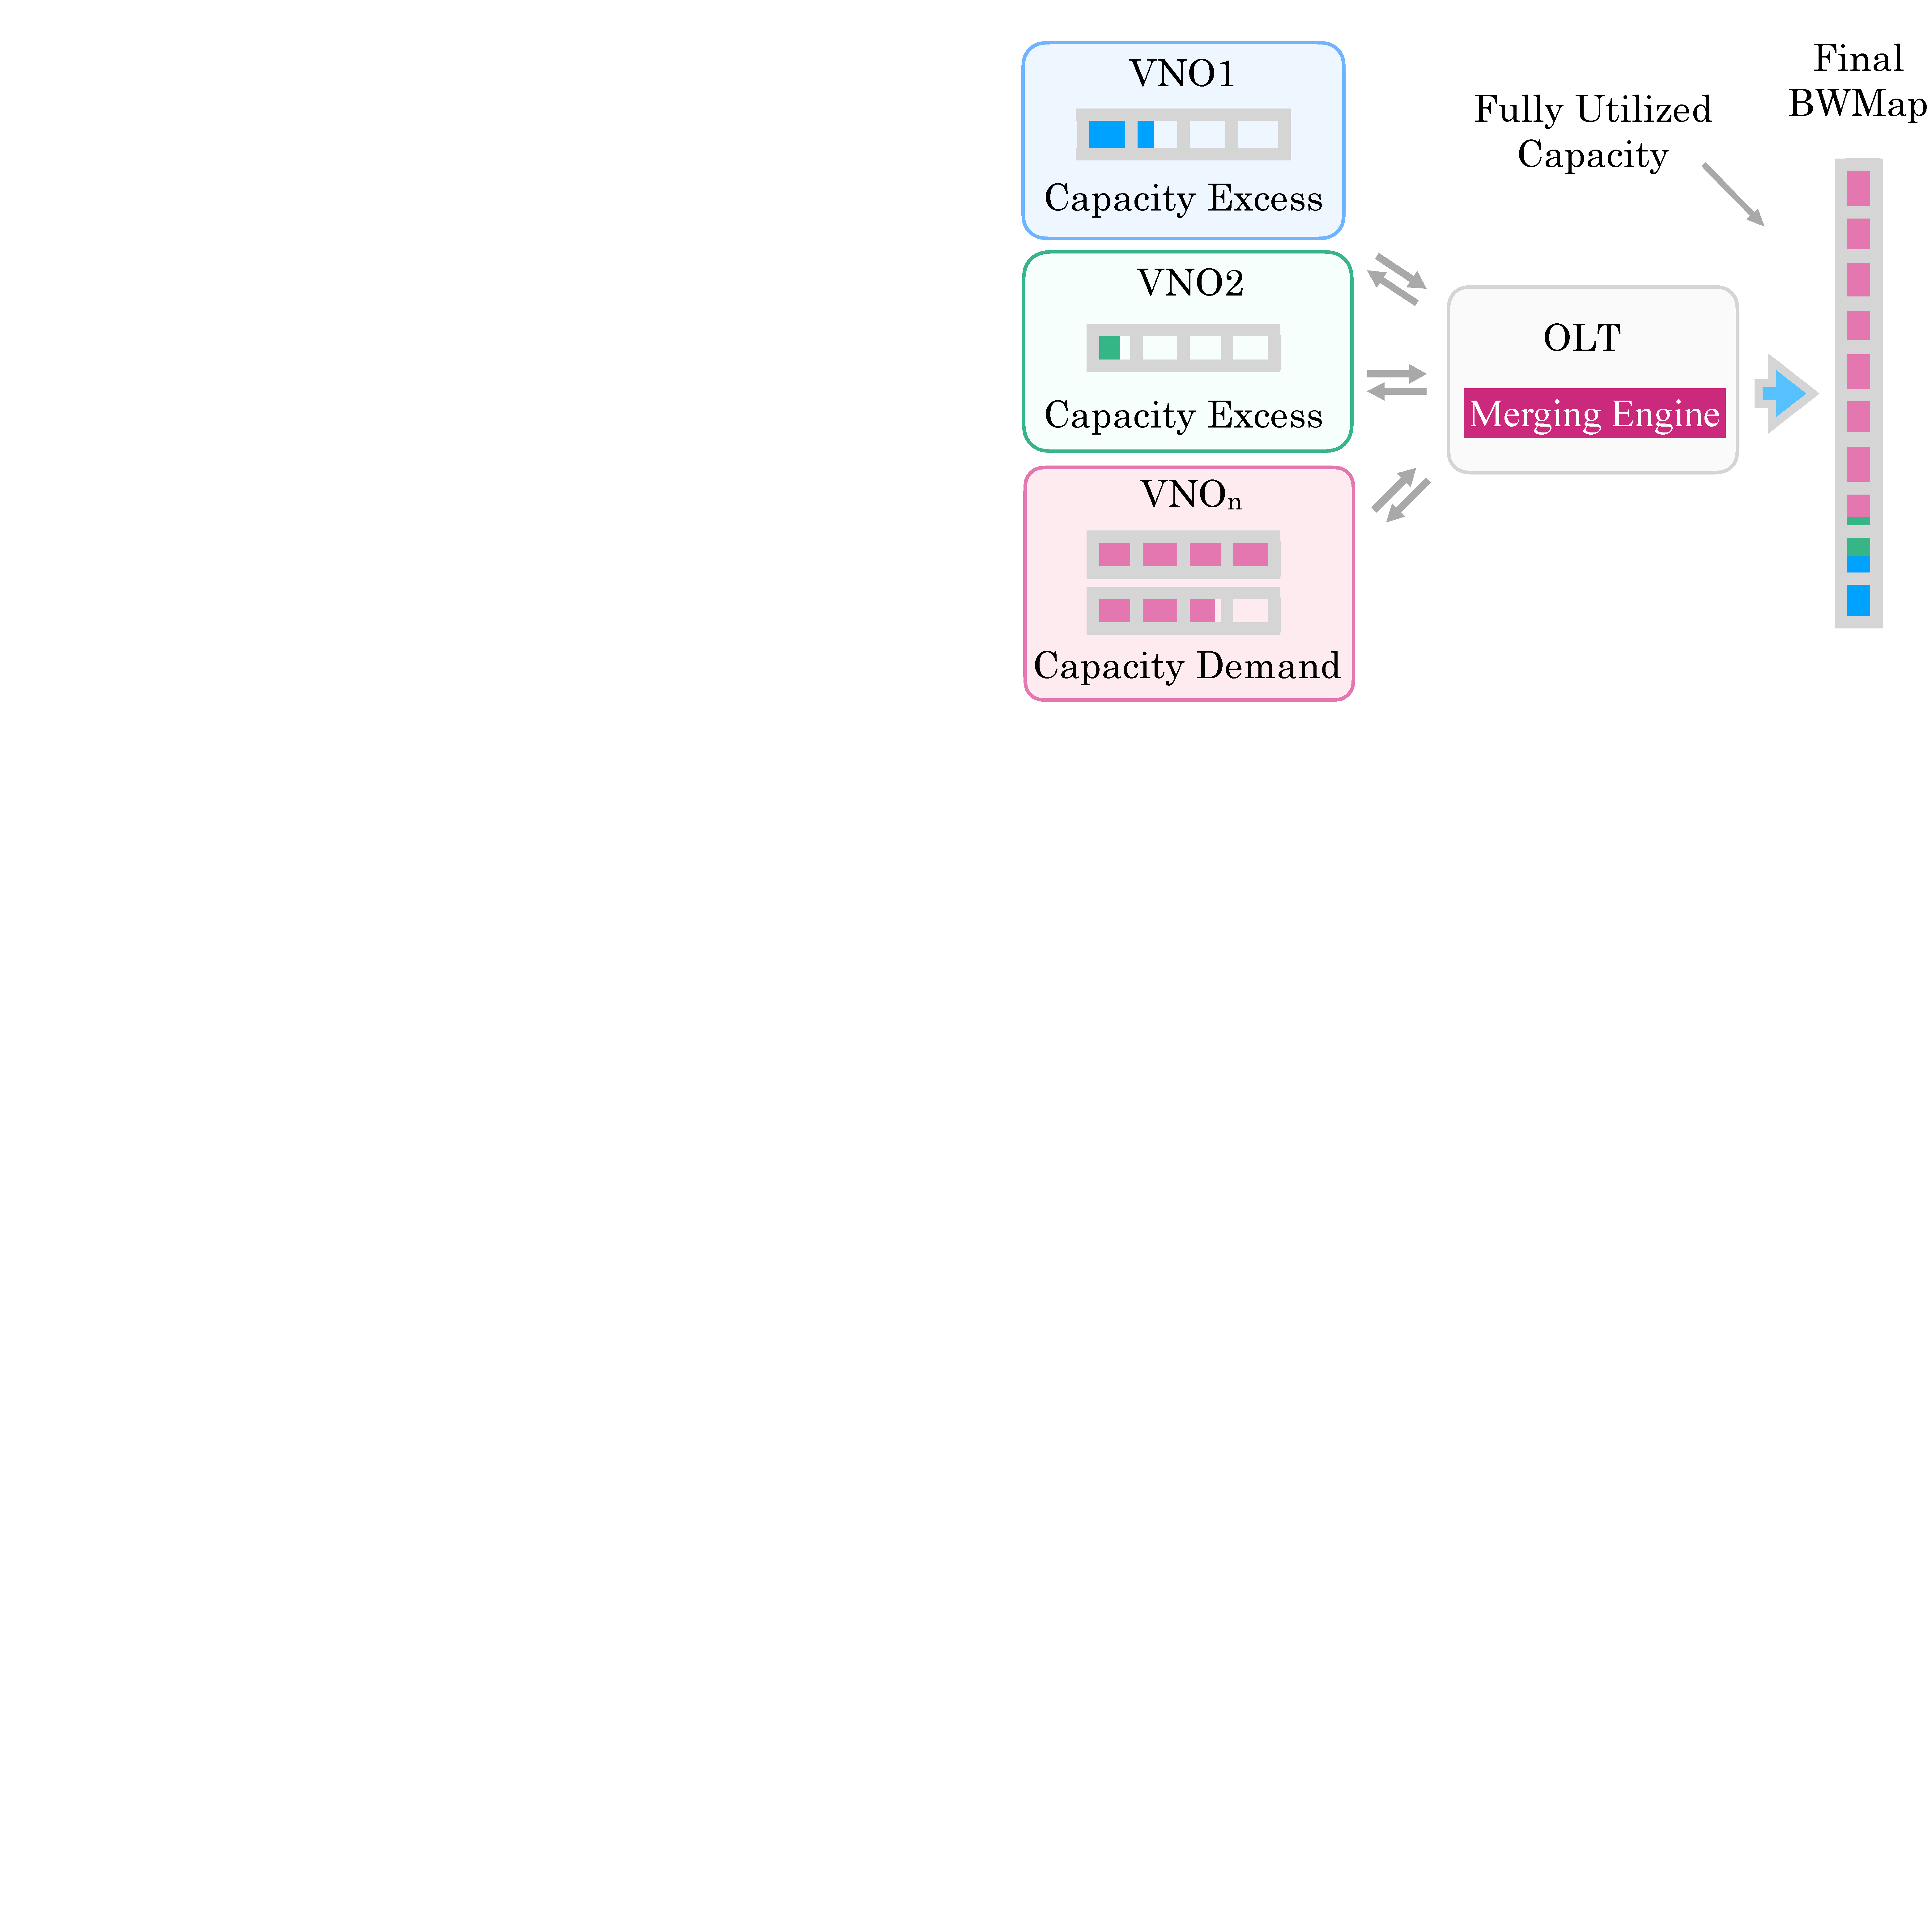
\includegraphics[width=\textwidth]{Figures/sharing.pdf}
\caption{Excess Sharing Policy}%
\label{sharing_p}
\end{subfigure}\hfill%
\caption{Inter-Operator Excess Capacity Sharing Policies}
\label{nonsharingvssharing_p}%
% \vspace{-9mm}
\end{figure}

To further investigate this, we have considered two merging policies:
\begin{itemize}
    \item Excess Non-Sharing Policy: in this policy (depicted in \figureautorefname~\ref{nonsharing_p}), each \acp{vDBA} shall produce \acp{vBMap} not exceeding their fixed dedicated share of the upstream frame: for example in the case of two \acp{VNO}, one could be allocated the first half of the upstream frame and the other the second half. The \ac{ME} layer simply concatenates the \acp{vBMap}. This simple policy does not allow the unused capacity of one \ac{VNO} to be shared with the other \acp{VNO}.
    
    \item Excess Sharing Policy: in this policy (depicted in \figureautorefname~\ref{sharing_p}), each \acp{vDBA} can act over the entire upstream frame, assigning capacity (assured, non-assured and best effort) up to the maximum amount that has been pre-negotiated with the \ac{PON} \ac{InP}. The \ac{ME} layer will then merge the \acp{vBMap} from all \acp{VNO} according to the following conditions:
        \begin{itemize}
            \item If all bandwidth grants can be accommodated, then no changes will be made to any of the \acp{vBMap}.
            
            \item If some bandwidth grants cannot be accommodated, the bandwidth grants of overloaded \acp{VNO} are to be reduced in order to be fitted in the next upstream frame. In order to reduce bandwidth grants, the \ac{ME} layer starts reducing best-effort traffic grants first. If still not enough, non-assured traffic bandwidth grants are also to be reduced. Assured capacity will always be allocated.
        \end{itemize}
\end{itemize}

The performance evaluation of the proposed \ac{DBA} virtualization is presented in \cite{Elrasad:17}. The simulation results show that it is possible to realize \ac{DBA} virtualization while not imposing considerable additional signaling delay to \ac{PON}'s capacity scheduling. The results also show that excess sharing policy has significantly superior network utilization (lower frame loss) compared to the excess non-sharing policy. Therefore the decision of the sharing policy could significantly improve the overall utilization of the network.

\section{Conclusions}

% \begin{boxbox}[colback=white]{Customizable scheduling as a technical enabler for \ac{PON} sharing}
% How to meet the technical requirements to enable fine-grained and dynamic optical network sharing?
% \end{boxbox}

In this chapter we introduced the concept of \ac{DBA} virtualization. The objective of \acp{vDBA} is to allow \acp{VNO} to implement their version of \ac{DBA} autonomous from the \ac{InP}. % The procedure of the bandwidth allocation starts with the \ac{OLT} forwarding the Buffer occupancy messages from \acp{ONU} to each \ac{vDBA}. Next, each \ac{vDBA} would issue the \ac{vBMap} for their \acp{ONU} using customized \acp{DBA} to fulfill their requirements. Finally, \acp{vDBA} send partial \ac{vBMap} to the \ac{ME} Layer to decide the final \ac{BMap}. 
Our proposed virtualization of the \ac{DBA} is included in the \ac{BBF} TR-402 standard and been patented~\cite{Nima-vDBA-patent}. This allows different \acp{VNO} to implement their flavor of the \ac{DBA}, providing them with the required flexibility to control the upstream scheduling, paving the way for the adoption of \acp{PON} as a primary transport network solution for new bandwidth-intensive services (\ac{5G}, Virtual reality, etc.). In this chapter, we have addressed the possibility of providing the required control to the \acp{VNO} by dedicating virtual and programmable instances of the \ac{DBA} algorithms. Therefore, each \ac{VNO} will operate a portion of the network, and their bandwidth allocation decision (referred to as \ac{vBMap}) is aggregated by the \ac{ME} in the final \ac{BMap}. Regarding the inter-operator excess capacity, two different approaches for the merging algorithm, namely excess sharing and excess non-sharing policies, have been studied with the excess sharing policy indicating significantly better results in terms of \ac{PON} utilization. The reported results show that the sharing capacity approach can enable true multi-tenancy while not imposing any significant delay to the \ac{PON} scheduling. 

\subsection{Contribution}
Giving \acp{VNO} the ability to schedule their entire capacity creates a new problem. If a \ac{VNO} has leftover capacity on any given frame, it would have no gain in leaving this unallocated, as the \ac{ME} would redistribute it to other \acp{VNO} which are likely to be its competitors. Thus its best strategy would always be to send a fully allocated \ac{vBMap} to the \ac{ME}. This constitutes a problem as it reduces the overall upstream \ac{PON} efficiency.


This challenge motivated the research question addressed in the next chapter of this dissertation, where we propose the monetization of the excess capacity of \ac{PON} slices using an auction mechanism. We enable the \acp{VNO} to trade their excess capacity in return for monetary compensation. The proposed market-based approach provides the absent sharing incentive for the \acp{VNO} and assures high network utilization.

The experimental results have been omitted from this chapter to retain the originality of this dissertation as the experiments have been carried out by other co-authors (accessible in \cite{Elrasad:17}). The author's contribution to this work includes developing the architecture for the \ac{DBA} virtualization, the \acp{vDBA}' interaction with the \ac{OLT} and the merging engine policy.

% \towrite{I think you should say that this work was carried out with multiple peope and your contribution was in the arcitecture and on the analysis of the vnos, inp relations. it's a way to justify not showing performance results but saying that his drives the rest of the work for next chapters}




% \subsection{Dissemination}

% \subsubsection{Peer-Reviewed}

%  \begin{enumerate}
%     \item M. Ruffini, A. Ahmad, S. Zeb, \textbf{\underline{N. {Afraz}}}, and F. Slyne, "The Virtual DBA: Virtualizing Passive Optical Networks to Enable Multi-Service Operation in True Multi-Tenant Environments," J. Opt. Commun. Netw., Jan. 2020.
    

%     \item A.~{Elrasad}, \textbf{\underline{N. {Afraz}}}, M.~{Ruffini} , ``Virtual Dynamic Bandwidth Allocation Enabling True PON Multi-Tenancy,'' in \emph{2017 Optical Fiber Communications Conference and Exhibition (OFC)}, March 2017, pp. 1--3.
%   \item \textbf{\underline{N. {Afraz}}}, F.~Slyne, M.~Ruffini, ``Full PON Virtulisation Supporting Multi-Tenancy Beyond 5G [Invited],'' in \emph{OSA Advanced Photonics Congress (AP) 2019 (IPR, Networks, NOMA, SPPCom, PVLED)}.\hskip 1em plus 0.5em minus 0.4em\relax Optical Society of America, 2019, p. NeT2D.2.
%  \end{enumerate}

  


%  \subsubsection{Patent}
%     \begin{enumerate}
%     \item M.~Ruffini, A.~Elrasad, \textbf{\underline{N. {Afraz}}}, ``System and {Method} for {Dynamic} {Bandwidth} {Assignment} (DBA) {Virtualization} in a {Multi}-{Tenant} {Passive} {Optical} {Network},'' Patent WO/2018/167\,318, Sep., 2018.
%     %   \item \bibentry{Nima-vDBA-patent}
%     \end{enumerate}


% \subsection{Implementation}
% Our \ac{vDBA} concept was demonstrated in \cite{8385950} on test bed incorporating a physical \acp{vDBA}, a set of emulated \acp{ONU}, a traffic generator and a multi-access edge computing node. The physical \ac{PON} was implemented on Xilinx VC709 FPGA boards, operating at symmetric 10Gb/s line rate.
% \label{test-bed}
% \begin{figure}[H]
% \centering
% 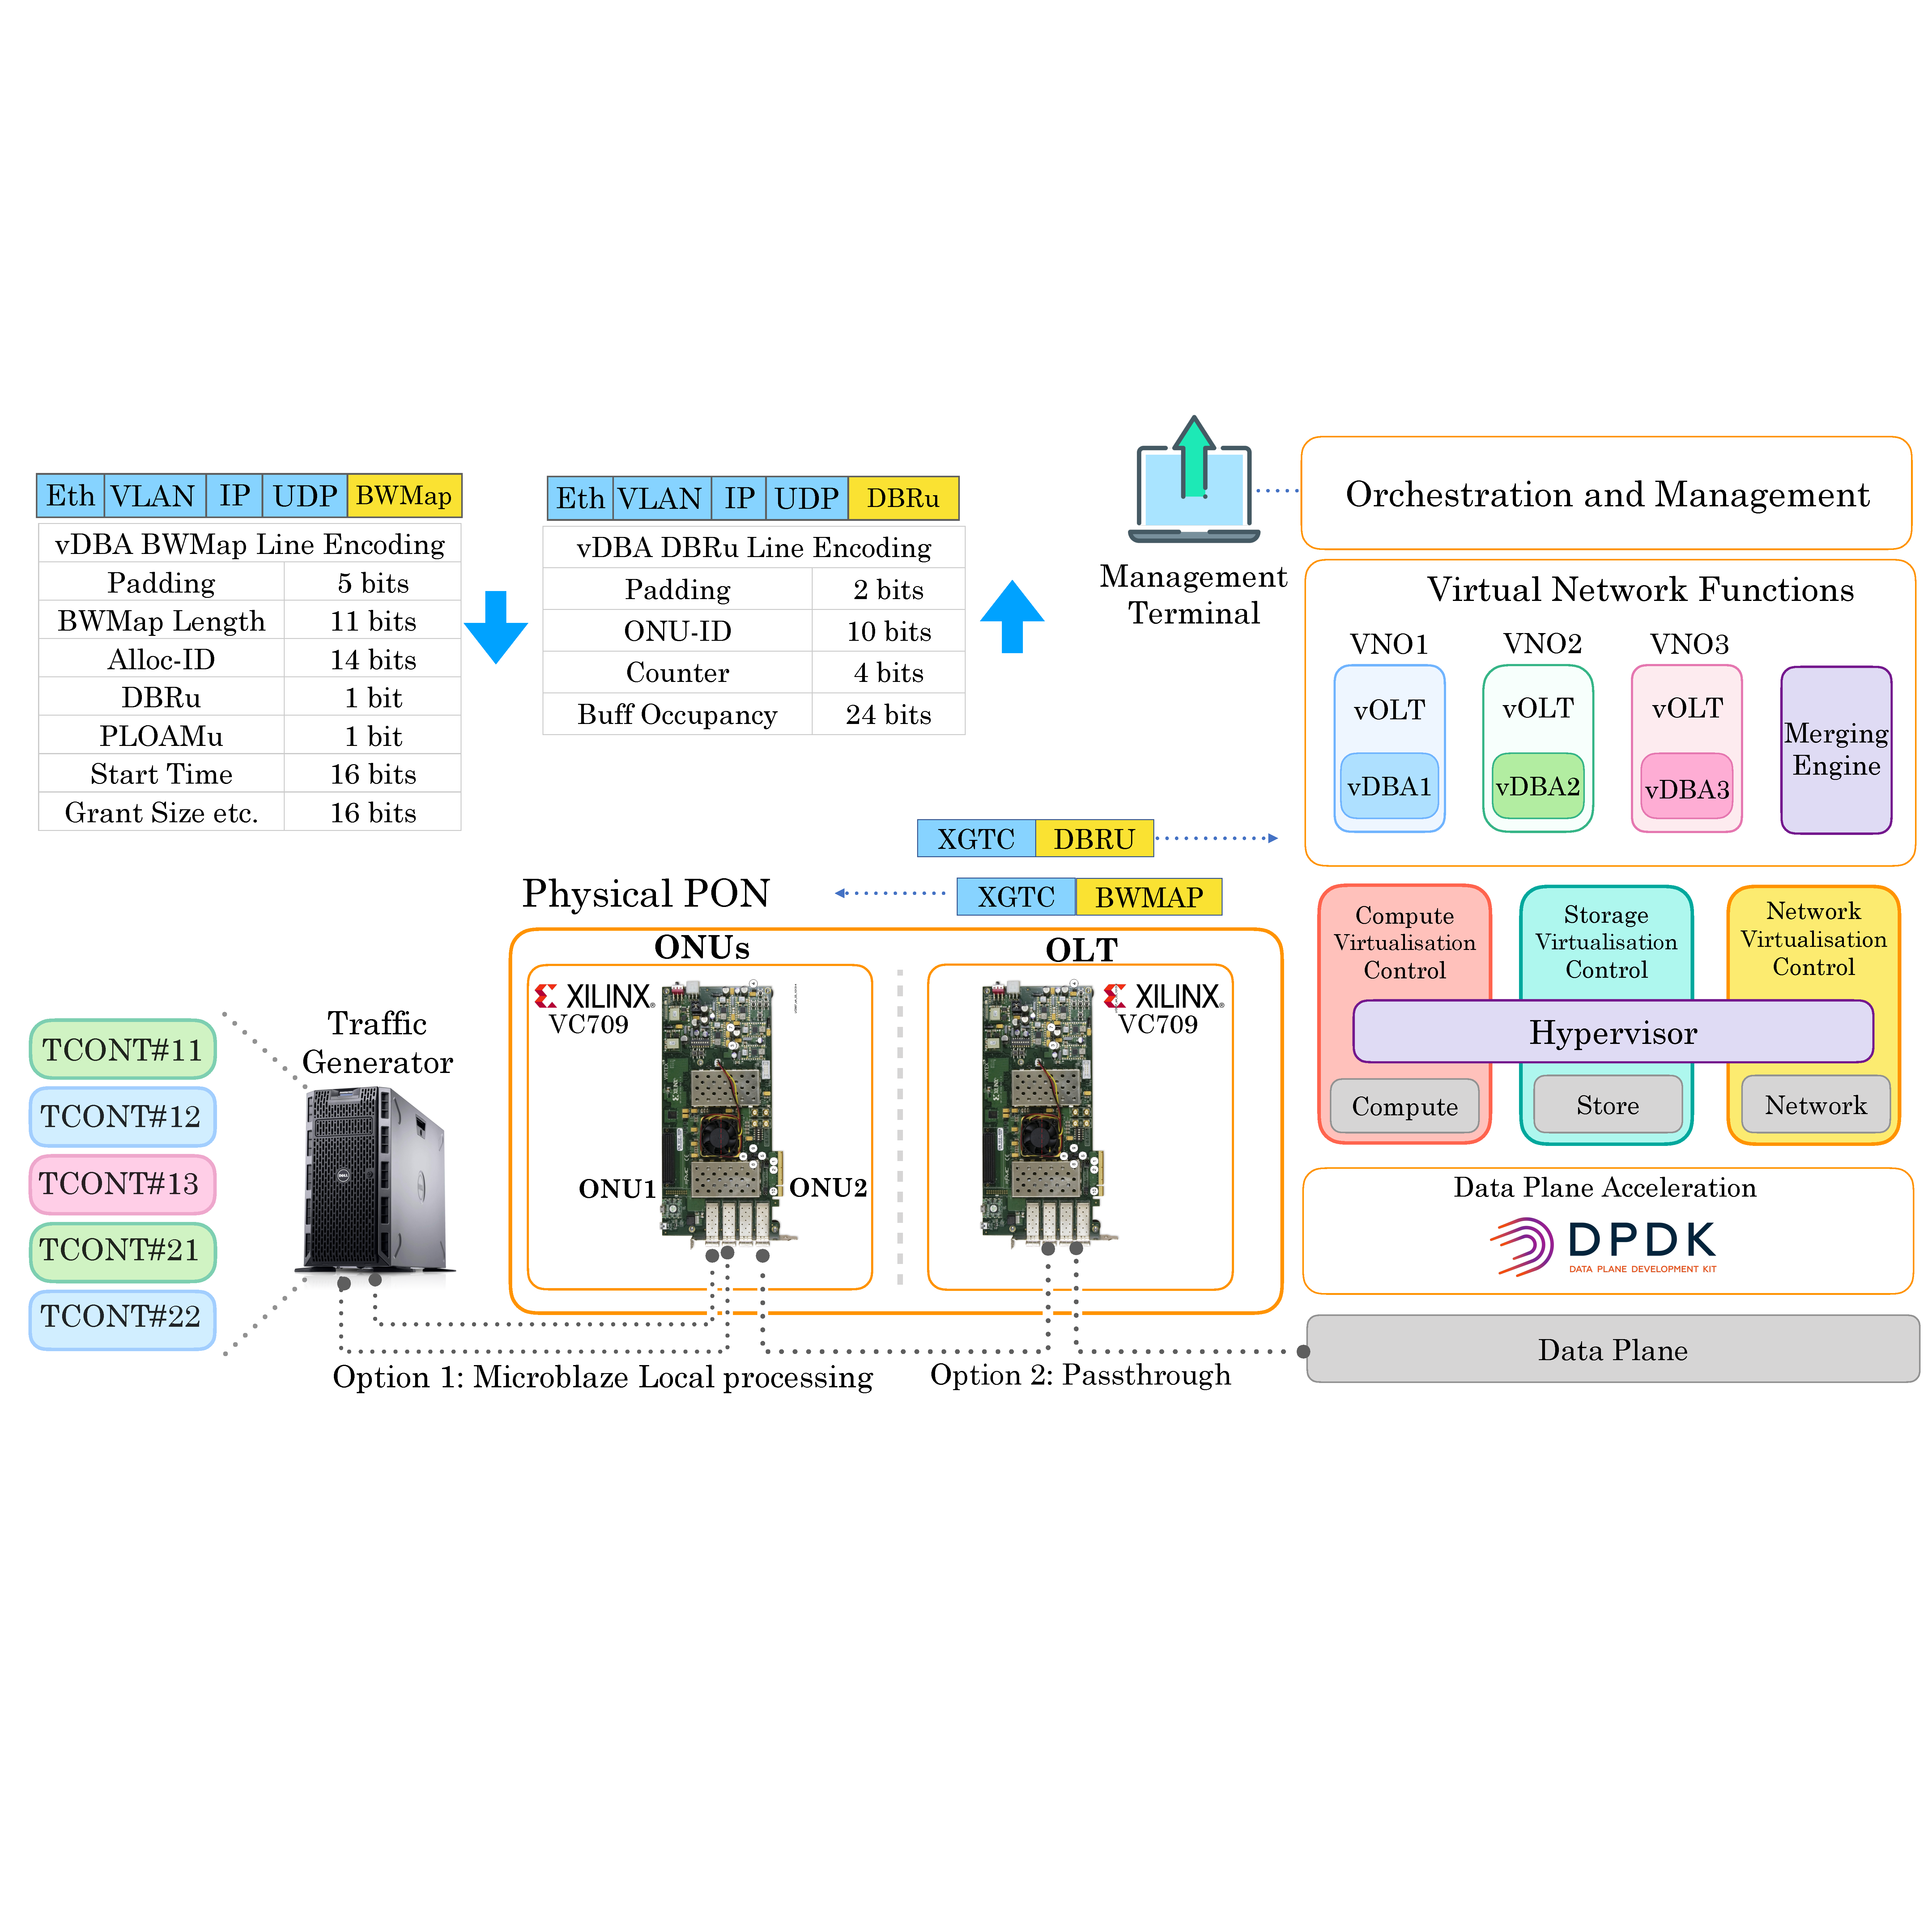
\includegraphics[width=\textwidth]{Figures/vdba_testbed_new.pdf}
% \caption{ \ac{vDBA} edge Compute stack}
% \end{figure}
% The \ac{PON} hardware and software virtualisation architecture is shown in \figureautorefname~\ref{test-bed}.
% The Multi-access Edge Computing (MEC) node hosted the \ac{ME} (ME) and the \ac{vDBA} functions for the Virtual Network Operators ( \acp{VNO} ), implemented as Virtual Network Functions. The \ac{ME} is the element that blends together all \ac{vBMap}s from the different \acp{VNO} so as to generate one physical \ac{BMap} allocation) and the SDN control plane. Due to the real-time critical nature of receiving and transmitting status report messages from the \acp{ONU} (called DBRUs) and \ac{BMap} data, our latest implementation \cite{slyne2018experimental},\cite{8606981} made advanced use of the Data Plane Development Kit (DPDK) toolkit to optimize the packet transfer through the physical host to and from the Virtual Network Functions. 
 


% Trinity patent declared as part of Broadband Forum protocols.


% A major funding investment by the Irish funding agency SFI, via the CONNECT Research Centre hosted in TCD, has resulted in intellectual property generated by an RPO, becoming pivotal to next-generation broadband networks. A Trinity patent has been declared as a standard-essential patent (SEP). That is a patent that claims an invention that must be used to comply with a technical standard.

% The Broadband Forum is the communications industry's leading organization focused on accelerating broadband innovation, standards, and ecosystem development. It is a non-profit industry organization composed of the industry's leading broadband operators, vendors, and thought leaders. As an example of their work Forum's flagship TR-069 CPE WAN Management Protocol has nearly 1 billion installations worldwide. Broadband Forum working groups collaborate to develop multi-service broadband packet networking specifications addressing architecture, device and service management, software data models, interoperability and certification in the broadband market.

% The forum has over 150 members including all the major global network operators including Vodafone, Telefonica and AT\&T as well as vendors including Ericsson, Nokia and Cisco. Interestingly however as well as Trinity only one other university is a member, namely the University of New Hampshire. Trinity's involvement has been solely due to the work of Prof Marco Ruffini , in the School of Computer Science and SFI Principal Investigator as part of the CONNECT Centre for future networks hosted in TCD. Marco's main research is in the area of 5G optical networks, where he carries out pioneering work on the convergence of fixed-mobile and access-metro networks, and on the virtualisation of next generation networks. It is his work in the latter area, that has piqued the interest of the BroadBand forum. So much so that some of Marco's key intellectual property has been declared as part of the TR-402 protocol "A Functional Model for \ac{PON} (Passive Optical Network) Abstraction Interface".

% In a little more technical detail, this IP defines a new system architecture, based software defined network technologies as required by operators. This is accomplished by disaggregating \ac{PON} functions into functional modules with open interfaces. The BBF's new \ac{PON} Abstraction Interface for Time-Critical Applications project, develops the architecture further by specifying a \ac{PON} abstraction interface for time-critical processing functions, such as Dynamic Bandwidth Assignment (DBA). This ground breaking concept has been encapsulated in a patent filed by Trinity entitled "System and Method for Dynamic Bandwidth Assignment (DBA) Virtualization in a Multi-Tenant Passive Optical Network" (ref: PCT/EP2018/056767).

% This technical protocol as defined by the forum is licensed to all the members but as TCD has declared the patent as being required for the standard, then those members that implement the standard require a licence from TCD. Such a patent patent is dubbed a "Standard Essential Patent" or SEP.

% The members of the broadband forum are shown below:





 
 
 
 


